\section{Polynomial Interpolation}

\begin{bigidea}
Given points $(t_0,y_0), \dots , (t_d,y_d)$, there exists a unique polynomial $p(t)$ of degree (at most) $d$ such that $p(t_k) = y_k$ for each $k=0,\dots,d$.
\end{bigidea}

\begin{definition}
Given $d+1$ points $(t_0,y_0), \dots , (t_d,y_d)$, polynomial interpolation with respect to the {\bf monomial basis} \cite[p.312]{MH} seeks a polynomial of the form
$$
p(t) = c_0 + c_1 t + \cdots + c_d t^d
$$
such that $p(t_k) = y_k$ for each $k=0,\dots,d$. The elements $1,t,t^2,\dots,t^d$ form the monomial basis of the vector space $\mathbb{P}_d$ of polynomials of degree less than or equal to $d$. Note that each point defines an equation
\begin{align*}
c_0 + c_1t_0 + \cdots + c_d t_0^d &= y_0 \\
c_0 + c_1t_1 + \cdots + c_d t_1^d &= y_1 \\
& \ \vdots \\
c_0 + c_1t_d + \cdots + c_d t_d^d &= y_d
\end{align*}
This yields a system of equations $A \bs{c} = \bs{y}$
$$
\begin{bmatrix}
1 & t_0 & \cdots & t_0^d \\
1 & t_1 & \cdots & t_1^d \\
\vdots & \vdots & \ddots & \vdots \\
 1 & t_d & \cdots & t_d^d
\end{bmatrix}
\begin{bmatrix} c_0 \\ c_1 \\ \vdots \\ c_d \end{bmatrix}
=
\begin{bmatrix} y_0 \\ y_1 \\ \vdots \\ y_d \end{bmatrix}
$$
The matrix
$$
A = \begin{bmatrix}
1 & t_0 & \cdots & t_0^d \\
1 & t_1 & \cdots & t_1^d \\
\vdots & \vdots & \ddots & \vdots \\
 1 & t_d & \cdots & t_d^d
\end{bmatrix}
$$
is called a {\bf Vandermonde matrix}. Solve the system $A \bs{c} = \bs{y}$ to find the coefficients
$$
\bs{c} = \begin{bmatrix} c_0 \\ c_1 \\ \vdots \\ c_d \end{bmatrix}
$$
\end{definition}

\begin{note}
The condition number of a Vandermonde matrix gets very large as the size of the matrix increases. This means that interpolation by the monomial basis is very sensitive to changes in the data for polynomials of large degree. For example, for $11$ equally spaced points $t_0=0,\dots,t_{10}=10$, the Vandermonde matrix $A$ is 11 by 11 and has condition number larger than $10^{12}$. Yikes!
\begin{center}
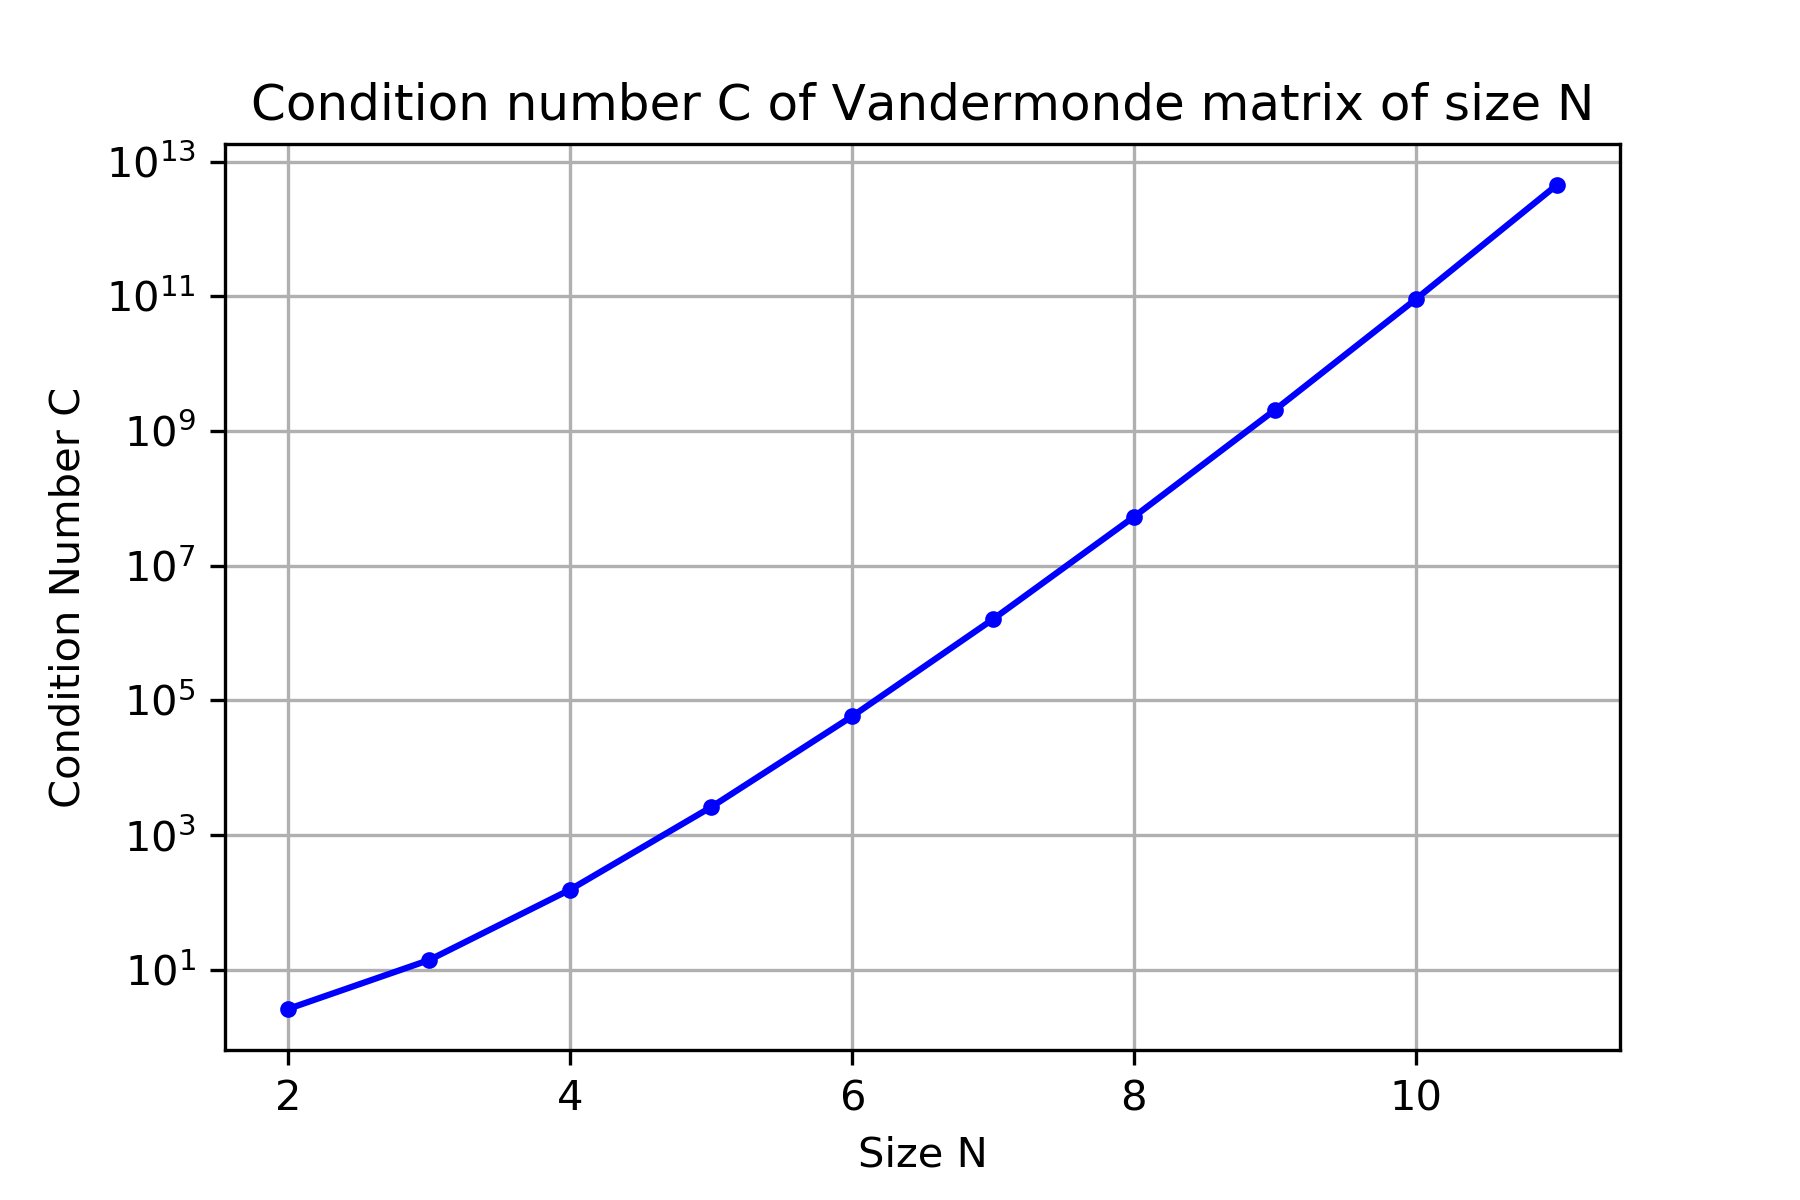
\includegraphics[width=4in]{01_05_img01.png}
\end{center}
\end{note}

\begin{proposition}
Consider $d+1$ data points $(t_0,y_0), \dots , (t_d,y_d)$ (such that $t_i \not= t_j$ for $i \not= j$). There exists a unique polynomial $p(t)$ of degree (at most) $d$ such that $p(t_k) = y_k$ for each $k=0,\dots,d$.

\begin{proof}
The Vandermonde matrix is invertible when the values $t_k$ are distinct therefore there is a unique solution of the system $A \bs{c} = \bs{y}$.
\end{proof}
\end{proposition}

\begin{definition}
Given $d+1$ points $(t_0,y_0), \dots , (t_d,y_d)$, {\bf Lagrange interpolation} \cite[p.315]{MH} seeks a polynomial of the form
$$
p(t) = c_0 \ell_0(t) + c_1 \ell_1(t) + \cdots + c_d \ell_d(t)
$$
where the {\bf Lagrange basis} $\ell_0(t),\dots,\ell_d(t)$ is given by
$$
\ell_k(t) = \frac{\prod_{j=0, j\not=k}^d (t - t_j)}{\prod_{j=0, j\not=k}^d (t_k - t_j)}
$$
The essential property of these polynomials is
$$
\ell_k(t_j) = \left\{ \begin{array}{cc} 1 & \text{ if } k = j \\ 0 & \text{ if } k \not= j \end{array} \right. \ , \ \ k,j=0,\dots,d
$$
Clearly $c_k = y_k$ for $k=0,\dots,d$ and so
$$
p(t) = y_0 \ell_0(t) + y_1 \ell_1(t) + \cdots + y_d \ell_d(t)
$$
\end{definition}

\begin{definition}
Given $d+1$ points $(t_0,y_0), \dots , (t_d,y_d)$, {\bf Newton interpolation} \cite[p.317]{MH} seeks a polynomial of the form
$$
p(t) = c_0 p_0(t) + c_1 p_1(t) + \cdots + c_d p_d(t)
$$
where the {\bf Newton basis} $p_0(t),\dots,p_d(t)$ is given by
\begin{align*}
p_0(t) &= 1 \\
p_1(t) &= t - t_0 \\
p_2(t) &= (t - t_0)(t - t_1) \\
 & \ \ \vdots \\
p_{d-1}(t) &= (t - t_0)(t - t_1)(t - t_2) \cdots (t - t_{d-1}) \\
\end{align*}
\end{definition}

\begin{note}
Recall that there is a unique polynomial $p(t)$ of degree (at most) $d$ which interpolates $d+1$ points $(t_0,y_0), \dots , (t_d,y_d)$ if the values $t_0,\dots,t_d$ are different. Therefore the monomial, Lagrange and Newton bases all produce the {\it same} result but computed and represented differently. 
\end{note}

\begin{example}
Find the interpolating polynomial for $(-1,1),(0,0),(1,1)$ using each of the monomial, Lagrange and Newton bases. We know the result is $p(t) = t^2$. Begin with monomial interpolation and setup the Vandermonde matrix and solve the linear system $A \bs{c} = \bs{y}$
$$
\left[ \begin{array}{rrr} 1 & -1 & \phantom{+}1 \\ 1 & 0 & 0 \\ 1 & 1 & 1 \end{array} \right]
\begin{bmatrix} c_0 \\ c_1 \\ c_2 \end{bmatrix}
=
\begin{bmatrix} 1 \\ 0 \\ 1 \end{bmatrix}
\ \
\Rightarrow
\ \
\bs{c} = \begin{bmatrix} 0 \\ 0 \\ 1 \end{bmatrix}
$$
and therefore $c_0 = c_1 = 0$ and $c_2 = 1$ and so $p(t) = t^2$. Now construct the Lagrange basis
\begin{align*}
\ell_0(t) &= \frac{(t - 0)(t - 1)}{(-1 - 0)(-1 - 1)} = \frac{t(t-1)}{2} \\
\ell_1(t) &= \frac{(t - (-1))(t - 1)}{(0 - (-1))(0 - 1)} = 1-t^2 \\
\ell_2(t) &= \frac{(t - (-1))(t - 0)}{(1 - (-1))(1 - 0)} = \frac{t(t+1)}{2}
\end{align*}
and the interpolating polynomial
$$
p(t) = y_0 \ell_0(t) + y_1 \ell_1(t) + y_2 \ell_2(t) = (1)\frac{t(t-1)}{2} + (0) (1-t^2) + (1) \frac{t(t+1)}{2} = t^2
$$
Now construct the Newton basis
\begin{align*}
p_0(t) &= 1 \\
p_1(t) &= t - (-1) = t + 1 \\
p_2(t) &= (t - (-1))(t - 0) = t^2 + t
\end{align*}
Each point yields an equation $p(t_k) = y_k$ for $k=0,1,2$ and so we solve the linear system
\begin{align*}
\left[ \begin{array}{ccc} 1 & 0 & 0 \\ 1 & t_1 - t_0 & 0 \\ 1 & t_2 - t_0 & (t_2-t_0)(t_2-t_1) \end{array} \right]
\begin{bmatrix} c_0 \\ c_1 \\ c_2 \end{bmatrix}
&=
\begin{bmatrix} 1 \\ 0 \\ 1 \end{bmatrix}
\\
\left[ \begin{array}{rrr} 1 & 0 & 0 \\ 1 & 1 & 0 \\ 1 & 2 & 2 \end{array} \right]
\begin{bmatrix} c_0 \\ c_1 \\ c_2 \end{bmatrix}
&=
\begin{bmatrix} 1 \\ 0 \\ 1 \end{bmatrix}
\ \
\Rightarrow
\ \
\begin{bmatrix} c_0 \\ c_1 \\ c_2 \end{bmatrix} = \left[ \begin{array}{r} 1 \\ -1 \\ 1 \end{array} \right]
\end{align*}
The interpolating polynomial is again
$$
p(t) = c_0 p_0(t) + c_1 p_1(t) + c_2 p_2(t) = 1 - (t+1) + t^2 + t = t^2
$$
\end{example}
